\chapter{Implementation and Testing}

\section{FileSync.py application}
Application goal explained in~\autoref{file-sync}
Appendix code~\autoref{apx:file-sync-code}

FileSync is a python application that will synchronize all files in a specified path, with all participants within the synchronization room.

\section{Application.py}
Application flow explained in~\autoref{sensor-application}

Device code~\autoref{apx:device-code}
\gls{PKG} code~\autoref{apx:pkg-code}

Main code~\autoref{apx:main-code}

\subsection{Packet Design}
Initialization packets are limited to the structure in~\autoref{fig:init_interest-data}.

Sensor packets are limited to the structure in~\autoref{fig:sensor_interest-data}.

Data packets have a \textit{MAX_NDN_PACKET_SIZE} of 8800 bytes.
\begin{description}
	\item[Init Interest] - 
  The initialization Interest seen in~\autoref{fig:init_interest-data}
  KeyLocator can be of type Name. 
  As described in the \gls{NDN} Packet Format~\cite{ndnpacketformat}, generally this field can be used to specify where to download the certificate used to sign the Interest.
  However, in our trust model we use this field to publish the requesters Name, i.e. the requesters public key. 
  This is very useful when using \gls{IBE} and \gls{IBS}.
	\item[Init Data] - 
  The Data response the the initialization Interest contains data with a structure defined in~\autoref{apx:msgBuf-code} and illustrated in~\autoref{fig:init_interest-data}.
	\item[Sensor Interest] -
	As in the initialization Interest the KeyLocator field is used to define the requesters Name. ~\autoref{fig:sensor_interest-data}
	\item[Sensor Data] - 
  The Data response to the Sensor Interest uses the same structure as the initialization Data. It is illustrated in~\autoref{fig:sensor_interest-data}
\end{description}

\begin{figure}[ht]
  \centering
  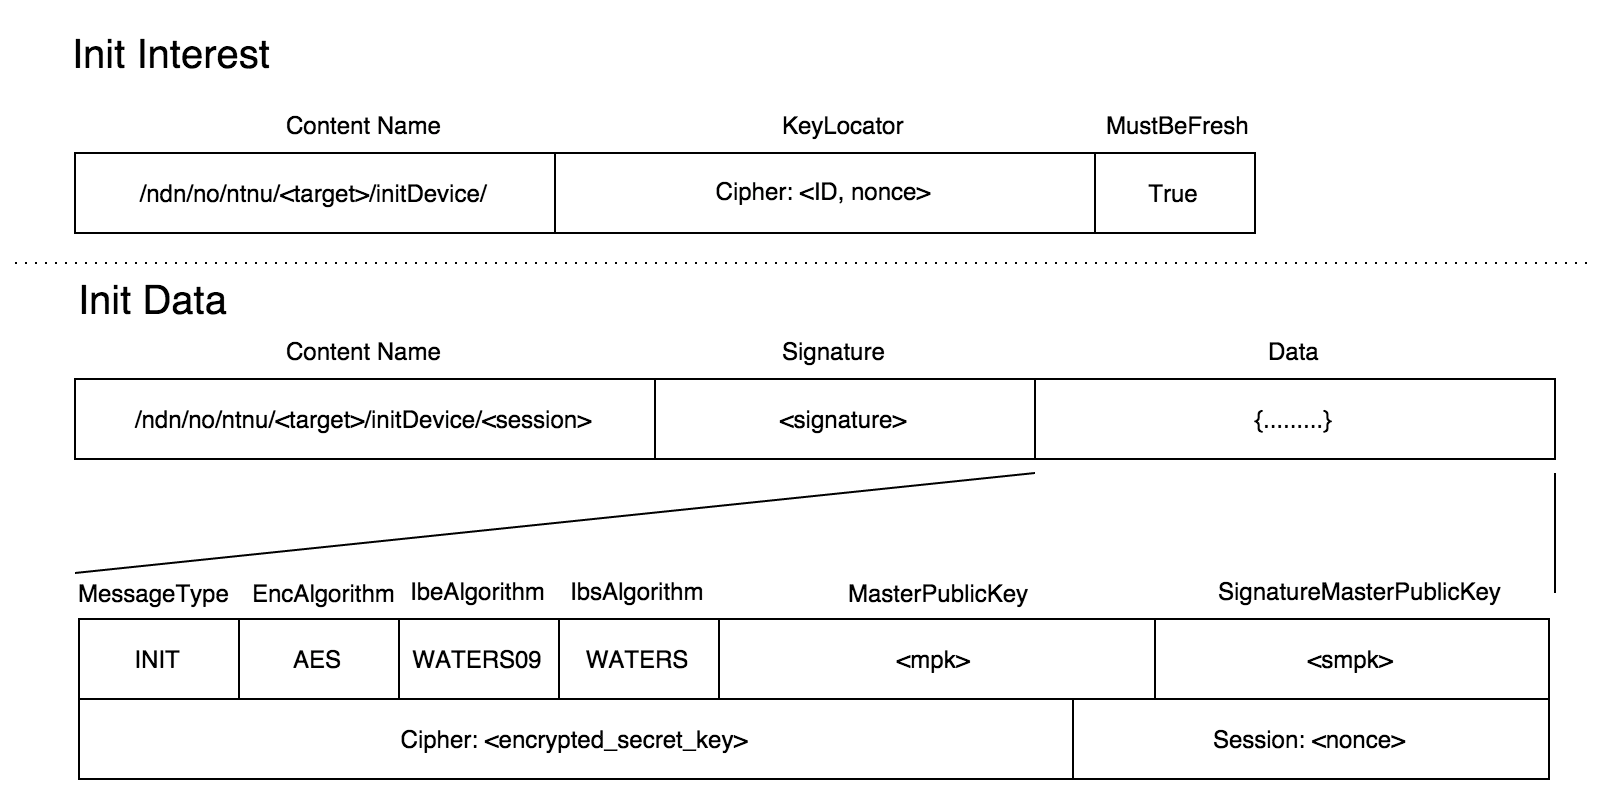
\includegraphics[width=1\textwidth]{init_interest-data.png}
  \caption{Initialization Interest and Data}
  \label{fig:init_interest-data}
\end{figure}

\begin{figure}[ht]
  \centering
  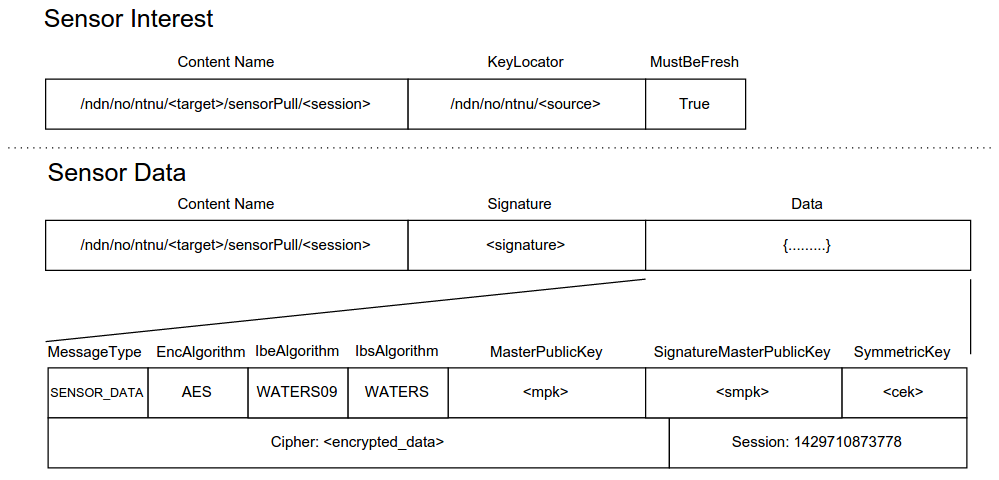
\includegraphics[width=1\textwidth]{sensor_interest-data.png}
  \caption{Sensor Interest and Data}
  \label{fig:sensor_interest-data}
\end{figure}

\section{IdentityBasedCrypto.py}
\gls{IBE} code~\autoref{apx:ibe-code} implements two \gls{IBE} schemes.

\begin{description}
  \item[Waters05]~\cite{DBLP:journals/iacr/Naccache05} that is a variant of Brent Waters \gls{IBE} scheme~\cite{DBLP:journals/iacr/Waters04}, but with smaller key size, hence more practical.
  \item[Waters09]~\cite{DBLP:conf/crypto/Waters09} that is also a fully secure implementation of \gls{IBE} scheme.
\end{description}